\chapter{Porting a \gls{ble} platform to Contiki \gls{os}}
\todo{ 5to10 pages} 
This chapter describes the initial task of choosing the hardware platform supporting \gls{ble} and porting Contiki \gls{os} to this platform. This task was a pre-requisite to the next task of testing detailed in chapter \ref{6Testing}. Section \ref{5HwPlt} explains the process of choosing a hardware platform and describes the chosen one. 

\section{\gls{ble} Hardware Platform} \label{5HwPlt}

As mentioned in section \ref{4Porting} Contiki has been ported to many hardware platforms. Since one of the main feature of Contiki is its communication stack capable of running in resource constrained systems, the primary aspect of a hardware platform is the \gls{mcu} and the communication interface. When choosing a hardware platform there are many other aspects that need to be considered as well. These include the availability of source code for peripheral drivers and examples, development environment (compiler, linker, programmer and debugger), development boards, documentation of the entire system and online forum for discussion.

Before this project, Contiki only supported wireless communication based on 802.15.4 physical layer. There are two types of platforms, namely platforms which consist of a discrete radio transceiver with a \gls{mcu} controlling it and platforms which consist of a \gls{soc} containing both the \gls{mcu} and radio transceiver in the same \gls{ic}. For including \gls{ble} support in Contiki, a hardware platform needed to be chosen and this process is explained in this section.

\subsection{Requirements of the hardware platform}
The \emph{mandatory} requirements for the platform would be:
\vspace{5pt}
\begin{easylist}[itemize]
& A \gls{soc} based platform.
& Must have a well supported and documented processor with good specifications.
& For a open source project such as Contiki, a free (and preferably open source) development toolchain must support the platform.
& Availability of well documented datasheet and user manual.
& Availability of an evaluation/development kit.
& Enough memory to accommodate Contiki and \gls{ble} stack’s requirements.
& Presence of basic peripherals such as timers and serial port required for Contiki.
\end{easylist}
\vspace{10pt}
\noindent
The non-mandatory, although \emph{nice to have} requirements for the platform would be:
\vspace{5pt}
\begin{easylist}[itemize]
& Presence of flexible power modes with low active and sleep power consumption.
& Availability of a good set of peripherals.
& Availability of \gls{ble} stack from the vendor, preferably with source code.
\end{easylist}
\vspace{10pt}

\subsection{Comparison and selection of the hardware platform}

With these requirements, based on the exhaustive comparison in \hyperref[AppendixA]{Appendix A} of the available \gls{soc} (\gls{ble}+\gls{mcu}) solutions available today, a platform based on nRF51822 from Nordic-Semiconductors would be a suitable option. As seen from the table in \hyperref[AppendixA]{Appendix A}, this platform would satisfy all the requirements mentioned above except for that the \gls{ble} stack would be available as a binary file, without the source code.

As shown in the table in \hyperref[AppendixA]{Appendix A}, recently many new promising \gls{ble} based \glspl{soc} have be released such as Quintic 9020, Dialog Semiconductor DA14580, Lapis MLA7105 and Broadcom BCM20732. From the limited technical information available about them, their technical specifications would be suitable for a project like this. But because of the limited documentation about them, scarce availability and nascent support they are not suitable.

\subsection{Overview of nrf51822 \gls{soc}}

nrf51822 is a \gls{soc} made by Nordic Semiconductor for developing \gls{ble} and 2.4 GHz based wireless systems \cite{nrf51822page}. Most of the specification of this \gls{soc} can be found in the table in \hyperref[AppendixA]{Appendix A}. The ARM Cortex M0 present is a 32 bit, 3 stage pipeline processor with Von Neumann architecture. It is designed for low silicon die size, low cost and power. It has an integrated \gls{nvic}  responsible for handling processor exceptions and peripheral interrupts. 

The development boards in the form of a USB dongle used for this thesis are called PCA10000. As seen in the figure \ref{pca10000}, the top side of PCA10000 contains nrf51822 at the centre, powered from the USB port through a regulator. This \gls{soc} is connected to a RGB led, a 16 MHz crystal, a 32.768  kHz crystal and a PCB antenna with its matching network. On the other side of the PCB is the SEGGER JLink Lite Cortex M unit. This can program and debug using the Serial Wire Debug (SWD) port of nrf51822. Another useful feature of this board is that the SEGGER JLink unit provides a serial port over USB with hardware flow control (HWFC) to the computer that this dongle is connected to. This serial port is connected to the UART port of nrf51822 \cite{PrithviR}.

\begin{figure}[h]
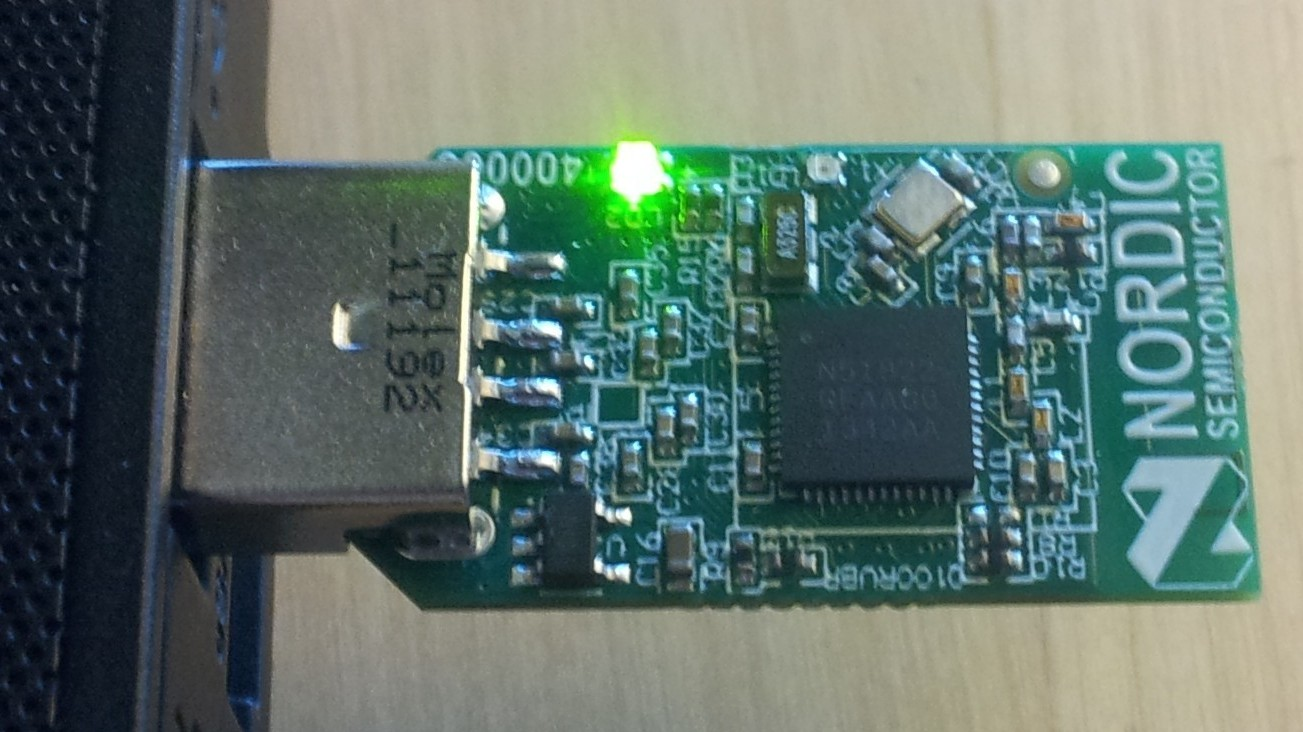
\includegraphics[width=\textwidth]{PCA10000}
\caption{PCA10000 development board}
\label{pca10000}
\end{figure} 

Nordic Semiconductor provides \gls{ble} stack as a precompiled and linked binary file called \emph{SoftDevices}. The SoftDevice is stored in a protected area in the flash memory and has access to a protected section of \gls{ram} memory, preventing unauthorized access by the application code. The SoftDevice can be accessed through a specified set of \gls{api} calls. These \glspl{api} are accessed by making a supervisor call to the processor causing a exception handler to run the SoftDevice. All calls are non-blocking, which means that the call will not stall the application making the call. And there are synchronous and non-synchronous calls, where the synchronous calls immediately return the result while the asynchronous calls start an operation that will send the result as an event to the application. A \gls{sdk} is also provided for nrf51822 which contains the peripheral drivers, examples, the interface header files for the SoftDevices and their documentation.
 


 
\todo{ development board, sniffer, master control panel, devzone}

From actively using this platform for many months, the subjective pros and cons of this platform would be as follows.

\noindent Pros:
\begin{easylist}[itemize]
& Large, mature and active community
& Support of open-source Eclipse and GNU-GCC development environment 
& Availability at low price
& Cortex M0 processor with competitive specs
& Support in mbed, an online open source development platform
& Support of supplementary tools such as nRF-Sniffer and android application 'Master Control Panel'
\end{easylist}
\vspace{10 pt} \noindent Cons:
\begin{easylist}[itemize]
& The \gls{ble} stack available as binary reducing flexibility
& \gls{sdk} not open for distribution
\end{easylist}

\section{Porting PCA10000 platform of nrf51822 to Contiki} \label{5Porting}
Contiki was initially developed in a Linux based operating system, although Windows is also supported now. The porting of PCA10000 platform to Contiki was done in Ubuntu 13.10. The compiler used is \todo{ ... explain all the other details of the development setup}

\subsection{Folder structure of Contiki}
When porting a new platform to Contiki, the three folders inside a Contiki distribution where additions need to be made are cpu, examples and platform. The content in these folders are as described below. The path of the Contiki distribution is in the path CONIKI.

\paragraph{CONTIKI/cpu}In this folder, all the files contain implementation which is solely dependent on the \gls{soc} is present. This includes the code for the processor abstraction, the drivers of the peripherals of the \gls{soc}, makefile with commands for compiling and linking the code, linker file and the documentation of these implementation. The boot-loader  or start-up code, if required is also present here. The peripheral drivers for peripherals such as timers and serial port must use the API format of Contiki so that the modules of Contiki using these peripherals can operate correctly. The exact implementations of these drivers is explained in section \ref{peripheralsContiki}. 

\paragraph{CONTIKI/platform} An \gls{soc} over time has increasing number of boards or systems that are based on it and these are referred as platforms in this folder. Every board has its own folder in this platform folder which contains files which contain implementation which is dependant on the particular board. These include the specification of the connections to the LEDs, buttons, sensors and serial ports power system, the clock sources, memories present and any other board specific details. Any peripheral driver implementation specific to the board is present here. The default project specifications such as the serial baud-rate and source and frequency of clock are defined here. The main function where the execution of the program starts and initialization of all the peripherals and modules used by Contiki happens is present here.

\paragraph{CONTIKI/examples} The examples folder contains all the files related to projects that are implemented using Contiki with any of the supported hardware platforms. The makefile where the make command is executed is present here. The compiled object and binary files are also stored here.

\subsection{Peripherals required for Contiki}\label{peripheralsContiki}
\subsubsection{Contiki Clock}
\subsubsection{R-Timer}
\subsubsection{LED(s)}
\subsubsection{Radio}
\subsubsection{Button(s)}
\subsubsection{Serial Port}

\subsection{Makefile structure of Contiki}

\textbf{Introduction to makefile and include.}
There are multiple makefiles present across different folders that are included in each other to form the complete makefile. In the most basic form these are the makefile in the example folder, `makefile.include' in the Contiki root folder, `makefile.TARGET' in the specific platform folder and `makefile.CPU' in the specific cpu folder, where TARGET and CPU are specific to the project. This structure by which this inclusion happens is illustrated better in \textbf{figure}.

Makefile where the project is present i.e. in the example folder
-Makefile.include in root CONTIKI directory
--Makefile indicating the target (if not already specified)
--Makefile of applications, if any are required
--Makefile of the target, present in the platform directory
---Makefile of the \gls{soc}, present in the cpu directory

The makefile in the example folder is where the make command is called. The operations that can be performed with this make command depends on the makefile. Usually the operations are cleaning (removing the object and binary files), compiling the source files into object files , linking these object files to create an executable file, creating a binary file from this executable file, uploading the binary to the \gls{soc} to start execution and so on. 

The makefile in the project specific example folder, the different project source files are specified and the `makefile.include' present in the root CONTIKI folder is added. `makefile.inlcude' glues together all the required components of Contiki and provides the default implementation of compiling and linking. The target makefile in the specific platform directory is included here. In `makefile.TARGET' the source files present in this directory are added, any Contiki modules required are added and the \gls{soc} makefile in the specific directory is added. The \gls{soc} 



